\documentclass[numsec,webpdf,modern,large,namedate]{oup-authoring-template}
\onecolumn
\usepackage{verbatim}
\usepackage{array}
\usepackage{booktabs}
\usepackage{fontspec}
\setmainfont{Libertinus Serif}
\begin{document}
\journaltitle{Journal of Language Evolution}
\copyrightyear{2026}
\pubyear{2026}
\appnotes{Paper}
\firstpage{1}
\title{Supplementary Material}
\author[1,$\ast$]{David M. Goldstein}
\author[2]{Shawn H. McCreight}
\author[3]{\'{E}va Buchi}
\author[4]{John P. Huelsenbeck}

\address[1]{\orgdiv{Department of Linguistics}, \orgname{University of California, Los Angeles}\orgaddress{\street{UCLA}, \postcode{90095-1543}, \state{California}}}
\address[2]{\orgdiv{Nytril LLC}, \orgaddress{\street{2904 Horsehead Bay Dr. NW}, \postcode{98335}, \state{Washington}}}
\address[3]{\orgdiv{Centre national de la recherche scientifique}, }
\address[4]{\orgdiv{Department of Integrative Biology}, \orgname{University of California, Berkeley}\orgaddress{\street{UC Berkeley}, \postcode{94720}, \state{California}}}


\corresp[$\ast$]{David M. Goldstein\href{email:dgoldstein@humnet.ucla.edu}{dgoldstein@humnet.ucla.edu}}

\maketitle
\section{Methods}
\label{PaperSections_Methods}
This section outlines the assumptions of the evolutionary models, the procedures used for parameter estimation, and the statistical framework for comparing alternative models of segmental evolution. 

\subsection{Phylogeny}
\label{PaperSections_Phylogeny}
We assume that the languages in our study group are related by an unknown evolutionary tree, or phylogeny, denoted $\Psi $. The phylogeny encodes both the topological relationships among the $\textit{N}$ sampled languages and either their divergence times or the amount of evolutionary change accumulated along each branch. 

\begin{figure*}[b]
\centering
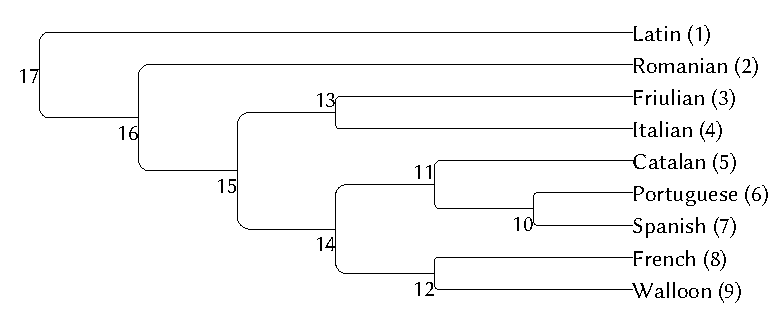
\includegraphics[width=352.688pt]{Figures/ExampleTree.pdf}
\caption{An example tree showing the relationships of $\textit{N}= 9$ languages.}
\label{ExampleTree}
\end{figure*}

Figure$~$\ref{ExampleTree} illustrates an example phylogeny for $\textit{N}= 9$ languages. In evolutionary biology, trees are described as consisting of ‘nodes’ and ‘branches.’ (Mathematicians instead use the terms ‘vertices’ and ‘edges’, respectively.) The terminal nodes, or tips, correspond to the sampled languages, while interior nodes represent divergence events. The tips are labeled $1, 2, \ldots , \textit{N}$, and the interior nodes are labeled $\textit{N}+ 1, \textit{N}+ 2, \ldots , 2\textit{N}- 1$ in preorder sequence (i.e., sequentially from the tips toward the root). The root node is assigned the label $2\textit{N}- 1$. For any node $i$, its immediate ancestor is denoted $\sigma (i)$. In Figure$~$\ref{ExampleTree}, for example, the ancestor of node 3 is $\sigma (3)= 13$. Branches connect the nodes of the tree and are represented as line segments in Figure$~$\ref{ExampleTree}. Each branch is labeled by its descendant node. In Figure$~$\ref{ExampleTree}, for example, the branch connecting nodes 13 and 14 is labeled 15. 

A phylogeny is an information-rich graph encoding both ancestry and divergence. Its topological component, denoted $\tau $, specifies the pattern of relationships among the languages. Figure$~$\ref{ExampleTree} indicates, for instance, that French and Walloon are each other's closest relatives. They share a more recent common ancestor with one another than with any other language in the tree (specifically, node 12 in Figure$~$\ref{ExampleTree}). The tree shown in Figure$~$\ref{ExampleTree} represents only one possible topology among many. For $\textit{N}= 9$ languages, there are 2,027,025 distinct rooted tree topologies. In general, the number of rooted trees is given by the product of the odd integers up to $2\textit{N}- 3$, namely $\mathbf{B}(\textit{N})= (2\textit{N}- 3)!!$$=$$1\times 3\times \ldots \times 2\textit{N}- 3$. We index these topologies as $\tau _1, \tau _2, \ldots , \tau _{\mathbf{B}(\textit{N})}$. The number of possible topologies grows extremely rapidly. For $\textit{N}= 60$ languages, for example, there are $5.86\times 1096$ distinct rooted trees. For comparison, the number of atoms in the observable universe is on the order of $10^{80}$. 

The interior nodes of the tree correspond to divergence events that occurred at specific times in the past. These divergence times are denoted $\mathbf{\textit{t}}= (\textit{t}_{\textit{N}+ 1}, \textit{t}_{\textit{N}+ 2}, \ldots , \textit{t}_{2\textit{N}- 1})$. All tip nodes are assigned time $\textit{t}= 0$. We describe below a stochastic model of language change operating along the branches of the tree. Such models include a rate parameter governing the tempo of evolution, denoted $\mu $, which represents the instantaneous rate of segmental substitution. In the absence of external calibration (such as a known divergence time) divergence times and substitution rates are not separately identifiable. A high substitution rate combined with a short divergence time produces the same expected amount of change as a low rate combined with a long divergence time. For two languages that diverged at time $\textit{t}$, the expected number of substitution events along the path connecting them is $\nu = 2\textit{t}\mu $. (The factor of two reflects the fact that the evolutionary path runs from one language to their common ancestor and then to the other language.) In the present study, each of the $2\textit{N}- 2$ branches is allowed to have its own substitution rate. Accordingly, the expected number of substitution events along the $i$th branch is $\nu = (\textit{t}_{\sigma _i}- \textit{t}_i)\times \mu _i$. Rather than estimating divergence times directly, we estimate the compound branch-length parameters $\nu _i$, measured in units of expected substitutions per segment. 

\subsection{Data}
\label{PaperSections_PhylogenyData}
Lexical similarities across languages provide evidence about their historical relationships. In this study, we draw on statistical methods developed in evolutionary biology, where phylogenetic relationships among species are inferred from shared morphological traits or from homologous DNA sequences sampled from the same gene across taxa. These methods rely on the assumption that the characters being compared are homologous---that is, that their similarity is attributable to common ancestry rather than independent innovation. In evolutionary biology, homology refers to similarity among traits attributable to descent from a common ancestor. As an illustration, consider the following DNA sequences sampled from three species:

\setlength{\tabcolsep}{0pt}
\begin{tabular}{b{72pt} b{360pt} }
Chimpanzee & AAGCTTCACCGGCGCAATTATCCTCATAATCGCCCACGGACTTACATCCT$\ldots$\\
Gorilla & AAGCTTCACCGGCGCAGTTGTTCTTATAATTGCCCACGGACTTACATCAT$\ldots$\\
Human & AAGCTTCACCGGCGCAGTCATTCTCATAATCGCCCACGGGCTTACATCCT$\ldots$\\
\end{tabular}

These sequences are partial mitochondrial DNA sequences reported by Gojobori  \citep{Hayasaka1988}. In the original study, the dataset comprised $\textit{N}= 12$ primate species and each sequence was 898 nucleotides in length. In phylogenetic analyses of DNA data, homology is assumed at two distinct levels. First, the sequences themselves must be homologous---that is, they must derive from the same gene in a common ancestor. At this level, homology is typically established through sequence similarity and synteny: the gene compared across species occupies the same genomic context, which means that it is located in the same or a closely corresponding position on the chromosome and flanked by the same neighboring genes. 

Second, fine-scale homology must be determined within the sequences. The DNA sequences shown above are presented in aligned form, where each column is treated as homologous across species. For example, the first column, which contains the nucleotide A in all three species, is assumed to correspond to a single ancestral position. Under this assumption, the common ancestor of gorillas, chimpanzees, and humans possessed a nucleotide at that position homologous to the aligned column. Fine-scale homology is inferred computationally in a procedure known as ‘alignment.’ Phylogenetic methods then proceed under the assumption that the inferred alignment correctly reflects true positional homology. 

Our treatment of linguistic data follows the general phylogenetic framework outlined above but differs from previous work in several important respects. As in most studies of linguistic phylogenetics, we restrict attention to the so-called ‘basic vocabulary’ \citep{Swadesh1952,Chang2015,Greenhill2021,Auderset2023,Heggarty2023}, as lexical items in this domain are comparatively resistant to borrowing. Unlike nearly all prior approaches, however, we base inference directly on phonemic word forms rather than on abstract cognate codings. For each concept in the dataset, homologous lexical items are grouped into a \textit{cognate class}. Within each class, word forms are represented phonemically using the International Phonetic Alphabet  \citep{IPA1999}. As an illustration, consider the cognate class for the concept ‘stone’:

\setlength{\tabcolsep}{0pt}
\begin{tabular}{b{72pt} b{14pt} b{14pt} b{14pt} b{14pt} b{14pt} b{14pt} b{14pt} }
Latin & p & - & e & t & r & a & m\\
Romanian & p & j & a & t & r & ə & -\\
Portuguese & p & - & ɛ & d & ɾ & ɐ & -\\
Spanish & p & j & e & d & ɾ & a & -\\
Catalan & p & - & e & d & ɾ & ə & -\\
French & p & j & ɛ & - & ʁ & - & -\\
Walloon & p & - & i & - & r & - & -\\
Friulian & p & j & e & - & r & e & -\\
Italian & p & j & ɛ & t & r & a & -\\
\end{tabular}

\begin{figure*}[b]
\centering
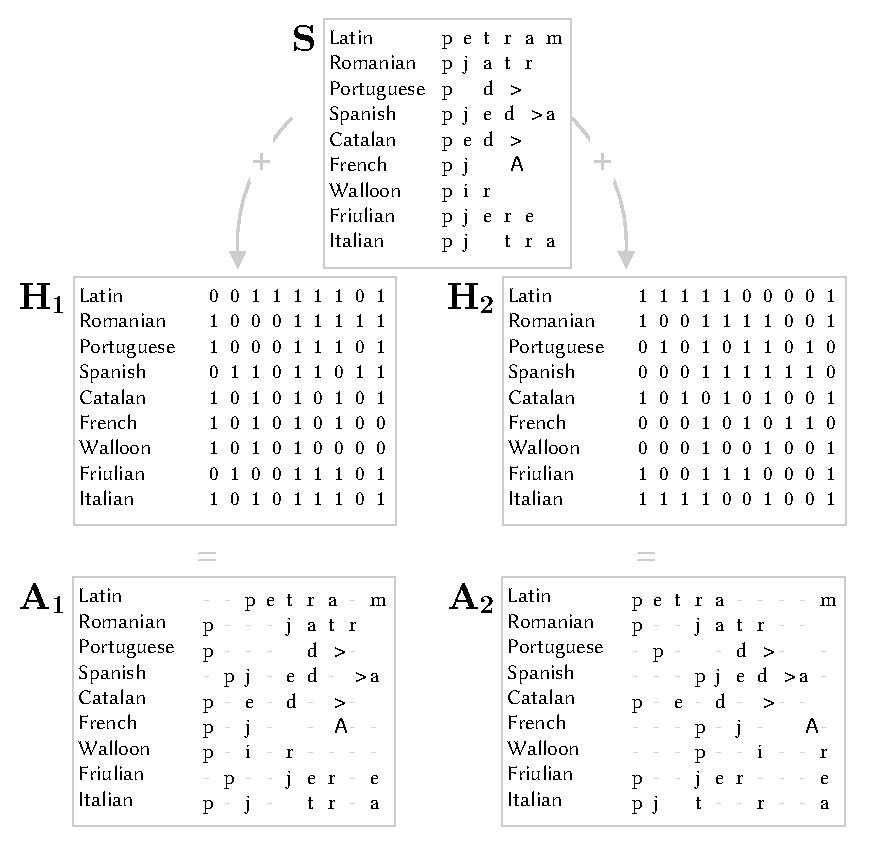
\includegraphics[width=400.425pt]{Figures/Alignment.pdf}
\caption{Alignments ($\mathbf{A}$) are formed from the observed segments ($\mathbf{S}$) and a homology map ($\mathbf{H}$). }
\label{Alignment}
\end{figure*}

The word for ‘stone’ in Latin, for example, is /petram/. The alignment matrix presupposes that fine-scale segmental homology has been specified. For instance, it treats the glide /j/ in Romanian, Spanish, French, Friulian, and Italian as homologous across these languages. Dashes indicate the absence of a segment homologous to those present in other forms at that alignment position. As discussed below, this alignment is not unique. Figure$~$\ref{Alignment} presents two alternative homology assignments. 

Formally, a segmental alignment, denoted $\mathbf{A}$, is obtained by combining the observed segmental strings with a specification of segmental homology. Let the segmental information for the $\textit{N}$ languages be denoted $\mathbf{S}= (\mathbf{s}_1, \mathbf{s}_2, \ldots , \mathbf{s}_{\textit{N}})$, where $\mathbf{s}_i$ represents the segmental string of the $i$th language. For the cognate class ‘stone’, the observed segmental strings are:

\setlength{\tabcolsep}{0pt}
\begin{tabular}{b{72pt} b{14pt} b{14pt} b{14pt} b{14pt} b{14pt} b{14pt} }
Latin & p & e & t & r & a & m\\
Romanian & p & j & a & t & r & ə\\
Portuguese & p & ɛ & d & ɾ & ɐ\\
Spanish & p & j & e & d & ɾ & a\\
Catalan & p & e & d & ɾ & ə\\
French & p & j & ɛ & ʁ & \\
Walloon & p & i & r &  & \\
Friulian & p & j & e & r & e\\
Italian & p & j & ɛ & t & r & a\\
\end{tabular}

For example, for Latin we have $\mathbf{s}_1= (petram)$. An alignment is determined by a homology map $\mathbf{H}$, which specifies which segmental positions correspond across languages. The alignment is therefore given by $\mathbf{A}= (\mathbf{S}, \mathbf{H})$. Figure$~$\ref{Alignment} provides two examples of alignments for ‘stone’ arising from different homology maps. 

Word forms are directly observable, whereas segmental alignments are not. Multiple homology assignments are often compatible with a given set of cognate forms, and the alignment for ‘stone’ shown above represents only one such possibility. In this study, we develop a statistical framework that treats segmental homology as a latent variable and integrates over its uncertainty. Rather than conditioning on a single alignment, the method considers all possible segmental alignments within a cognate class, weighting each by its posterior probability under the model. Inference is therefore averaged over alignment uncertainty rather than predicated on a fixed homology assignment. 

\subsection{Segmental evolution model}
\label{PaperSections_PhylogenyModel}
We model the evolution of cognate word forms along the branches of a phylogenetic tree as a sequence of segmental substitutions, insertions, and deletions. Substitution events are described by a continuous-time Markov process whose state space consists of the phonemic segments in the inventory. Central to this process is a rate matrix specifying the instantaneous rate of change between all ordered pairs of states. For illustration, consider a simplified model with five segments as states. The instantaneous transition rates can be represented in tabular form as follows:

\setlength{\tabcolsep}{0pt}
\begin{tabular}{b{56pt} b{32pt} b{32pt} b{32pt} b{32pt} b{32pt} }
\specialrule{0pt}{0pt}{1pt}
 & \multicolumn{5}{l}{To}\\
 & A & B & C & D & E\\
\specialrule{0.25pt}{0pt}{0pt}
A & $q_{AA}$ & $q_{AB}$ & $q_{AC}$ & $q_{AD}$ & $q_{AE}$\\
B & $q_{BA}$ & $q_{BB}$ & $q_{BC}$ & $q_{BD}$ & $q_{BE}$\\
From   C & $q_{CA}$ & $q_{CB}$ & $q_{CC}$ & $q_{CD}$ & $q_{CE}$\\
D & $q_{DA}$ & $q_{DB}$ & $q_{DC}$ & $q_{DD}$ & $q_{DE}$\\
E & $q_{EA}$ & $q_{EB}$ & $q_{EC}$ & $q_{ED}$ & $q_{EE}$\\
\end{tabular}



In this table, $q_{ij}\geq 0 (i\neq j)$ denotes the instantaneous rate of change from segment $i$ to segment $j$. The diagonal elements $q_{ii}$ are defined so that each row of the matrix sums to zero, i.e., $q_{ii}= - \sum _{j\neq i}{q_{ij}}$. Since these diagonal entries are negative, the quantity -$q_{ii}$ can be interpreted as the total rate at which the process leaves state $i$. In matrix notation, the substitution process is summarized as:

\begin{align}
\mathbf{Q}= \{q_{ij}\}= \left(\begin{array}{ccccc}
q_{AA} & q_{AB} & q_{AC} & q_{AD} & q_{AE}\\
q_{BA} & q_{BB} & q_{BC} & q_{BD} & q_{BE}\\
q_{CA} & q_{CB} & q_{CC} & q_{CD} & q_{CE}\\
q_{DA} & q_{DB} & q_{DC} & q_{DD} & q_{DE}\\
q_{EA} & q_{EB} & q_{EC} & q_{ED} & q_{EE}\\
\end{array}\right) \beta 
\end{align}

The scalar parameter $\beta $ rescales the matrix so that the equilibrium-weighted average substitution rate equals 1.0. Under this normalization, a branch length equals the expected number of substitutions per segment along that branch. 

A continuous-time Markov process admits a straightforward probabilistic interpretation. When the process occupies state $i$, the waiting time until the next substitution event is exponentially distributed with rate parameter -$q_{ii}$. Conditional on a substitution occurring, the probability that the next state is $j$ (for $i$ ≠ $j$) is $- q_{ij}/ q_{ii}$. Several quantities of interest follow directly from the rate matrix $\mathbf{Q}$. For example, the probability of transitioning from state $i$ to state $j$ over an interval of length $\nu $ is obtained by matrix exponentiation, $\mathbf{P}(\nu )= e^{\mathbf{Q}\nu }$. The process also admits a stationary, or equilibrium, distribution $\pi $, which represents the long-run probability of observing each state. This distribution is characterized as the solution to $\pi \mathbf{Q}= \mathbf{0}$. Both the transition probabilities and the equilibrium distribution enter into the likelihood calculation described below. 

Insertions and deletions of individual segments occur at rates $\lambda  and \mu $, respectively. The long-term behavior of the process depends critically on the relationship between these rates. If $\lambda > \mu $, insertions occur more frequently than deletions on average and word lengths increase without bound. Conversely, if $\lambda < \mu $, deletions dominate and word forms shrink progressively, eventually collapsing to length zero. 

The TKF91 model of DNA sequence evolution permits single nucleotides to be inserted and deleted at rates $\lambda  and \mu $ \citep{Thorne1991}. To formalize this process, Thorne et al. introduced a representation in which adjacent nucleotides are connected by invisible links. Each nucleotide is associated with the link immediately to its right and the left-most position is preceded by a special link known as the immortal link. Insertions occur to the right of an existing link and generate a new nucleotide together with a new link. Deletions remove a nucleotide and its associated link, but the immortal link itself is never deleted. This construction prevents the process from going extinct, even when $\lambda < \mu $, because a new nucleotide (and its link) can always be inserted to the right of the immortal link. 

The TKF91 model assumes that the insertion rate is strictly less than the deletion rate $(\lambda < \mu )$, which ensures that sequence length has a stationary distribution. Under this condition, the equilibrium distribution of sequence length is geometric with parameter $\lambda / \mu $. We adopt this constraint in the present study. The model implemented here is in fact identical to TKF91 with respect to insertions and deletions. It differs only in the substitution component. Whereas TKF91 employs a four-state nucleotide substitution process, we replace it with a continuous-time Markov model defined over the segmental inventory. 

The combined substitution and insertion--deletion process can be described as follows. Consider a sequence of length $L$, with $L_i$ instances of segment type $i$. The waiting time until the next evolutionary event (substitution, insertion, or deletion) is exponentially distributed with rate parameter: 

\begin{align}
r= - \sum _i{(L_iq_{ii})}+ L\lambda + (L- 1)\mu 
\end{align}

Conditional on an event occurring, the probability that it is a substitution equals $- \sum _i{(L_iq_{ii})}/ r$, the probability of an insertion equals $L\lambda / r$, and the probability of a deletion equals $(L- 1)\mu / r$. Since insertions and deletions operate on links that define positional homology, the alignment map $\mathbf{H}$ crucially becomes an explicit parameter of the model rather than a fixed input. 

\subsection{Bayesian estimation of model parameters}
\label{PaperSections_BayesianParameters}
Model parameters are estimated within a Bayesian framework. Inference is based on the posterior distribution of the parameters, obtained via Bayes’ rule:

\begin{align}
\textit{P}(Parameter(s) | Observations)= \frac{\textit{P}(Observations | Parameter(s)) \textit{P}(Parameter(s))\textit{P}(Observations)}{\textit{P}(Observations)}
\end{align}

In words, the posterior distribution conditional on the observations is proportional to the likelihood [\hbox{$[\textit{P}(Observations | Parameter(s))]$}] multiplied by the prior distribution [\hbox{$[\textit{P}(Parameter(s))]$}] and normalized by the marginal likelihood [\hbox{$[\textit{P}(Observations)]$}]. 

In this study, parameters include:

\setlength{\tabcolsep}{0pt}
\begin{tabular}{b{72pt} b{20pt} b{288pt} }
$\tau _1, \ldots , \tau _{\mathbf{B}(\textit{N})}$ &  & Tree Topologies\\
$\nu _1, \ldots , \nu _{\mathbf{B}(\textit{N})}$ &  & Branch-length parameters\\
$\textit{$\theta$}$ &  & Parameters associated with the rate matrix $\mathbf{Q}$\\
$\lambda , \mu  (\lambda < \mu )$ &  & Insertion and deletion rates\\
$\mathbf{H}$ &  & The map describing the alignment of the segments\\
\end{tabular}

Prior distributions are assigned to all parameters (see Table 1). The joint posterior distribution of the parameters is therefore:

\begin{align}
\textit{P}(\tau , \nu , \textit{$\theta$}, \lambda , \mu \vert \mathbf{S})= \frac{\textit{P}(\mathbf{S}\vert \tau , \nu , \textit{$\theta$}, \lambda , \mu ) \textit{P}(\tau , \nu , \textit{$\theta$}, \lambda , \mu )\textit{P}(\mathbf{S})}{\textit{P}(\mathbf{S})}
\end{align}

We highlight that the likelihood is marginalized over all possible segmental alignments: 

\begin{align}
\textit{P}(\mathbf{S}\vert \tau , \nu , \textit{$\theta$}, \lambda , \mu )= \sum _{\mathbf{H}}{\textit{P}(\mathbf{S}\vert \tau , \nu , \textit{$\theta$}, \lambda , \mu , \mathbf{H}) \textit{P}(\mathbf{H})}
\end{align}

Since the summation extends over all admissible alignment maps, inference does not condition on any single alignment being correct. Similarly, the marginal likelihood integrates over all possible parameter values:

\begin{align}
\textit{P}(\mathbf{S})= \sum _{\tau }\int _{\nu }\int _{\textit{$\theta$}}\int _{\lambda < \mu }{\textit{P}(\mathbf{S}\vert \tau , \nu , \textit{$\theta$}, \lambda , \mu ) \textit{P}(\tau , \nu , \textit{$\theta$}, \lambda , \mu ) \textit{d}\nu  \textit{d}\textit{$\theta$} \textit{d}\lambda  \textit{d}\mu }
\end{align}

The integrals represent integration over branch lengths, substitution-model parameters, and insertion-deletion rates, subject to the constraint $(\lambda < \mu )$. The likelihood itself is computed on a per-word basis using the dynamic programming algorithm of  \citet{Lunter2003}, which conditions on a specific alignment. Although the posterior distribution can be expressed analytically, the high-dimensional summations and integrals required for exact evaluation are intractable. We therefore approximate the joint posterior distribution numerically using Markov chain Monte Carlo (MCMC). 

\subsection{Markov chain Monte Carlo}
\label{PaperSections_MCMC}
Markov chain Monte Carlo (MCMC) provides a numerical method for approximating the posterior distribution of model parameters. The goal is to construct a Markov chain whose state space consists of parameter values and whose stationary distribution coincides with the posterior distribution of interest.  \citet{Metropolis1953} and  \citet{Hastings1970} describe general procedures for constructing such chains. Once stationarity has been reached, successive samples from the chain constitute dependent but asymptotically valid draws from the posterior distribution. We implement the Metropolis--Hastings algorithm as follows:

Let the current state of the chain be denoted $\textit{$\theta$}$. If this is the initial iteration, initialize $\textit{$\theta$}$, for example by drawing from the prior distribution.

Propose a new state, denoted $\textit{$\theta$}' $, by generating a random vector $u$ from a specified proposal distribution and defining $\textit{$\theta$}' = h(\textit{$\theta$}, u)$. Let $q(\textit{$\theta$}\rightarrow \textit{$\theta$}' )$ denote the proposal density for the forward move and $q(\textit{$\theta$}' \rightarrow \textit{$\theta$})$ the corresponding reverse-move density.

Compute the Metropolis--Hastings acceptance probability:

$$
R= \min (1, \frac{f(\textit{$\theta$}' \vert \mathbf{X})f(\textit{$\theta$}\vert \mathbf{X})}{f(\textit{$\theta$}\vert \mathbf{X})}\times \frac{f(\textit{$\theta$}' )f(\textit{$\theta$})}{f(\textit{$\theta$})}\times \frac{q(\textit{$\theta$}' \rightarrow \textit{$\theta$})q(\textit{$\theta$}\rightarrow \textit{$\theta$}' )}{q(\textit{$\theta$}\rightarrow \textit{$\theta$}' )})
$$This quantity equals the product of the likelihood ratio, prior ratio, and proposal ratio.Draw a uniform random variable $u$ from the interval (0,1). If $u< R$, accept the proposal and set $\textit{$\theta$}= \textit{$\theta$}' $. Otherwise, reject the proposal and retain the current state.

Repeat from step 1.The proposal mechanisms employed here are standard in phylogenetic inference, including the LOCAL move for updating tree topologies and branch lengths \citep{Larget1999}. The distinctive feature of the present analysis is the inclusion of proposals for segmental alignments. We implement the alignment proposal strategy described by \citet{Lunter2005b}. 

In practice, the Markov chain is run for a large number of iterations. At each iteration, a proposed move is either accepted or rejected, which produces a stochastic sequence of parameter states. States are recorded at regular intervals. In our analysis, every 100th iteration was retained. Posterior summaries are derived from the retained samples. For example, the proportion of samples in which a particular alignment appears provides a Monte Carlo estimate of its posterior probability and the proportion supporting a given tree topology provides a corresponding estimate for that topology. Marginal posterior distributions for continuous parameters are estimated from the empirical distribution of sampled values. 

\subsection{Model comparison}
\label{PaperSections_MCMCComparison}
In Bayesian inference, parameter estimation proceeds from the joint posterior distribution, which we approximate using the Metropolis--Hastings algorithm. In many applications, however, the primary goal is to compare competing models and determine which provides the better account of the observed data. Bayesian model comparison is based on the marginal likelihoods of the models. Consider two linguistic models, $\textit{M}_1$ and $\textit{M}_2$, with marginal likelihoods $\textit{P}(\mathbf{S}\vert \textit{M}_1)$ and $\textit{P}(\mathbf{S}\vert \textit{M}_2)$, respectively, computed for the same dataset. The ratio of these marginal likelihoods is the Bayes factor:

\begin{align}
\textit{BF}_{12}= \frac{\textit{P}(\mathbf{S}\vert \textit{M}_1)\textit{P}(\mathbf{S}\vert \textit{M}_2)}{\textit{P}(\mathbf{S}\vert \textit{M}_2)}
\end{align}

The Bayes factor quantifies the relative support for the two models. A value greater than one favors $\textit{M}_1$, whereas a value less than one favors $\textit{M}_2$. Unlike frequentist model comparison, Bayesian inference does not rely on \textit{p}-values. Instead, Bayes factors are interpreted either directly or on a logarithmic scale.  \citet{Jeffreys1961} proposed the following conventional guidelines:

\setlength{\tabcolsep}{0pt}
\begin{tabular}{b{72pt} b{72pt} b{216pt} }
$\textit{BF}$ & $log_{10}$$\textit{BF}$ & Interpretation\\
\specialrule{0.5pt}{0pt}{0pt}
1$-$3.2 & 0$-$0.5 & Not worth a bare mention\\
3.2$-$10 & 0.5$-$1 & Substantial\\
10$-$100 & 1$-$2 & Strong\\
$>$100 & $>$2 & Decisive\\
\end{tabular}

Bayesian model comparison automatically accounts for model complexity through integration over parameter space. More complex models distribute prior probability mass over a higher-dimensional space, which effectively penalizes unnecessary parameters. Consequently, no additional correction for model size, such as a null distribution comparison, is required.

A practical challenge in Bayesian model comparison is the numerical approximation of marginal likelihoods. Several strategies are available. One approach constructs a Markov chain that moves between models of differing dimensionality via reversible-jump MCMC \citep{Green1995}. Another approach estimates marginal likelihoods using path-sampling or thermodynamic integration, in which a series of MCMC chains explores intermediate distributions between the prior and posterior \citep{Lartillot2006,Xie2010}. 

Three models of segmental evolution are compared in this study. The first is isomorphic to the Jukes--Cantor model \citep{Jukes1969} and assumes equal rates of change between all segment pairs. The second corresponds to the Felsenstein model \citep{Felsenstein1981}, in which substitution rates are proportional to the stationary frequency of the destination state. The third, the Natural Class Model, partitions segments into ten articulatorily defined classes and estimates separate rates for changes within classes and between classes.

\subsection{Cognates Sets}
\label{PaperSections_UsedCognates}
The dataset contains 102 cognate sets comprising 918 word forms and 79 distinct phonemic segments distributed across 98 concepts: all, and, at, belly, black, blood, bone, dog, dry, ear, earth, egg, eye, feather, fingernail, fire, five, flower, foot, four, fruit, full, good, grass, green, head, I, if, in, knee, leaf, liver, long, louse, meat, moon, mountain, mouth, narrow, near, new, night, not, old, one, other, rain, red, river, round, salt, sea, seed, skin, sky, star, stone, tail, there, thick, thin, three, come, cut, drink, fall, fight, flow, hear, hold, know, laugh, lieasinabed, play, say, see, sew, sing, sleep, smell, squeeze, stand, swell, think, turn, wash, tongue, tooth, tree, warm, water, what, when, wind, woman, year, you (pl.), and you (sg.). 

\subsection{Workflow}
\label{PaperSections_Workflow}
The first stage of the experiment involved constructing a reusable dictionary of IPA segment definitions. The files IPA.nytril and Segments.nytril define segment classes, with each segment represented as an instance containing its IPA symbol (e.g., /ŋ/) and a set of phonological attributes (e.g., vowel, sibilant, fricative). These files were designed for reuse in future experiments and by other researchers. 

\begin{figure*}[b]
\centering
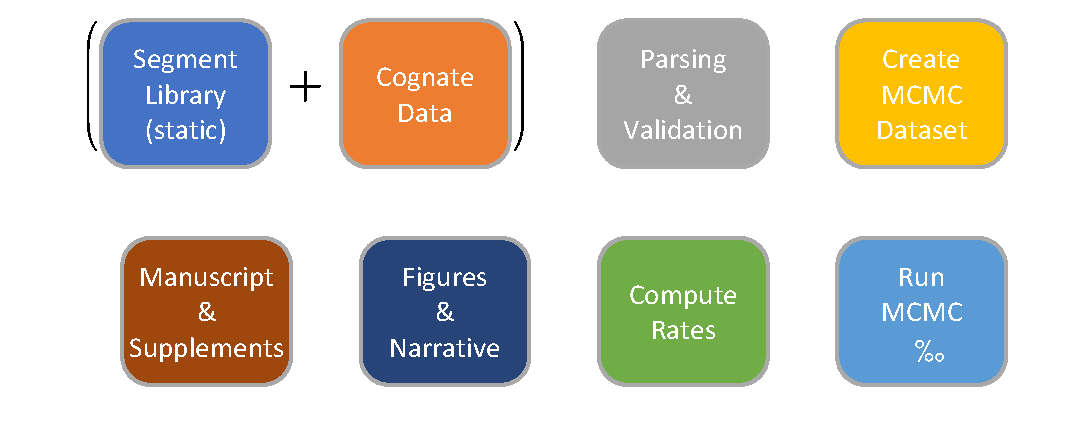
\includegraphics[width=495.9pt]{Figures/Workflow.pdf}
\caption{The workflow of the experiment.}
\label{Workflow}
\end{figure*}

The next stage consisted of assembling the cognate word forms. These are stored as strings in nytril source files organized by concept and language. Each string contains UCS code points encoding the IPA symbols for its segments, which allows for consistent copying across sources. Dashes between IPA symbols provide an initial vertical alignment of segments. Syllable stress marks may appear in the strings but are ignored in the present analysis. Although the word files are grouped by part of speech (e.g., Nouns.nytril, Adjectives.nytril), this organization is purely editorial. During processing, all forms are aggregated and reorganized programmatically. 

The strings are then decoded and converted into arrays of VocalSegment objects. Since IPA characters may consist of multiple Unicode code points and include combining diacritics, all strings are normalized to Unicode Form C (NFC) prior to comparison. This ensures that diacritics occupy consistent relative positions across strings. After parsing, each word is reconstructed from its object representation to verify fidelity to the original encoding. The segment objects are subsequently grouped into words and organized by concept, cognate class, and language, yielding a structured representation of the full dataset. 

Diagnostic tables and visualizations are then generated to inspect the data from multiple perspectives. These diagnostics facilitate detection of alignment errors, encoding inconsistencies, or structural anomalies. Once the dataset has been validated, an experiment snapshot is generated. This process produces a directory of nytril and JSON files that serve as input to the program TongueTwister. 

TongueTwister performs the MCMC analysis, which may run for several days and produces tree files and associated output. The resulting files are then processed by TongueTwisterReader, which aggregates posterior summaries and generates formatted output files in nytril format. Finally, a nytril-based program reads the processed output and produces the tables, charts, and figures included in the manuscript. These graphical outputs are integrated with narrative text to generate the final paper and presentation materials. Figure$~$\ref{Workflow} provides a schematic overview of the workflow. 


\bibliographystyle{abbrvnat}
\bibliography{main}

\end{document}

